\clearpage
\myparagraph{First \olly example: a=1.2 and b=3.4}
\myindex{\olly}

Let's load the example into \olly:

\begin{figure}[H]
\centering
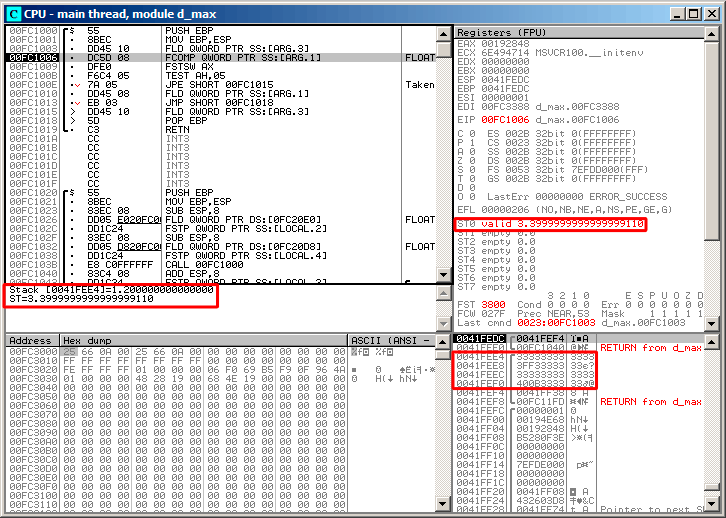
\includegraphics[scale=\FigScale]{patterns/12_FPU/3_comparison/x86/MSVC/olly1_1.png}
\caption{\olly: first \FLD is executed}
\label{fig:FPU_comparison_case1_olly1}
\end{figure}

Current arguments of the function: $a=1.2$ and $b=3.4$ (We can see them in the stack: two pairs of 32-bit values).
$b$ (3.4) is already loaded in \ST{0}.
Now \FCOMP is being executed. 
\olly shows the second \FCOMP argument, which is in stack right now.

\clearpage
\FCOMP is executed:

\begin{figure}[H]
\centering
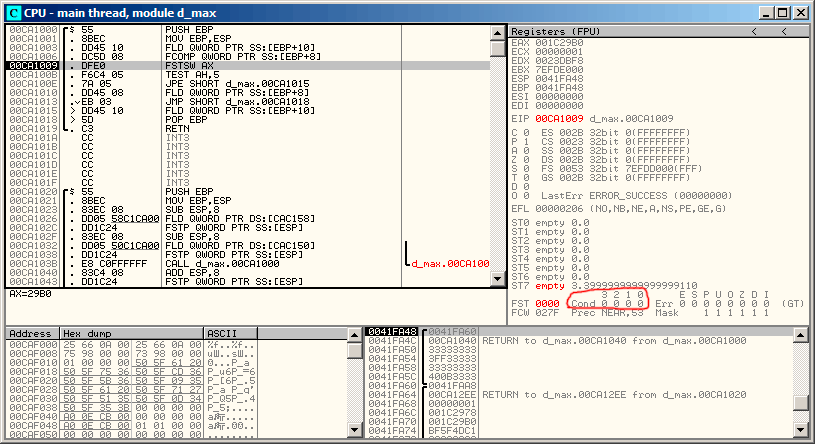
\includegraphics[scale=\FigScale]{patterns/12_FPU/3_comparison/x86/MSVC/olly1_2.png}
\caption{\olly: \FCOMP is executed}
\label{fig:FPU_comparison_case1_olly2}
\end{figure}

We see the state of the \ac{FPU}'s condition flags: all zeroes.
The popped value is reflected as \ST{7}, it was written earlier about reason for this: 
\myref{FPU_is_rather_circular_buffer}.

\clearpage
\FNSTSW is executed:
\begin{figure}[H]
\centering
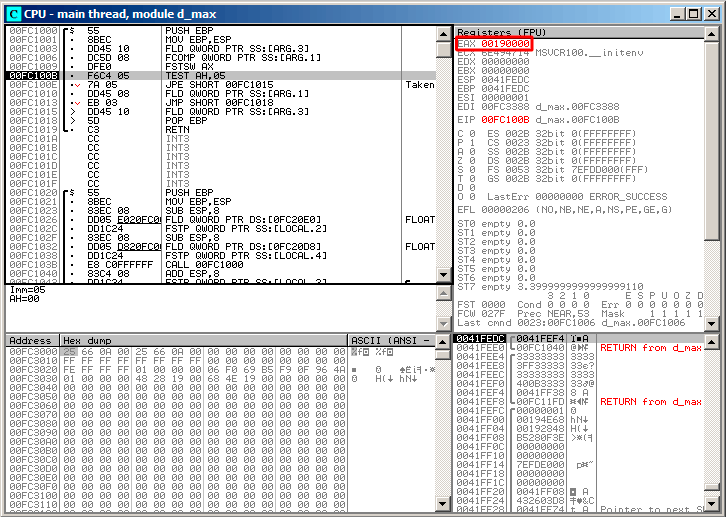
\includegraphics[scale=\FigScale]{patterns/12_FPU/3_comparison/x86/MSVC/olly1_3.png}
\caption{\olly: \FNSTSW is executed}
\label{fig:FPU_comparison_case1_olly3}
\end{figure}

We see that the \GTT{AX} register contain zeroes: indeed, all condition flags are zero.
(\olly disassembles the \FNSTSW instruction as \INS{FSTSW}---they are synonyms).

\clearpage
\TEST is executed:

\begin{figure}[H]
\centering
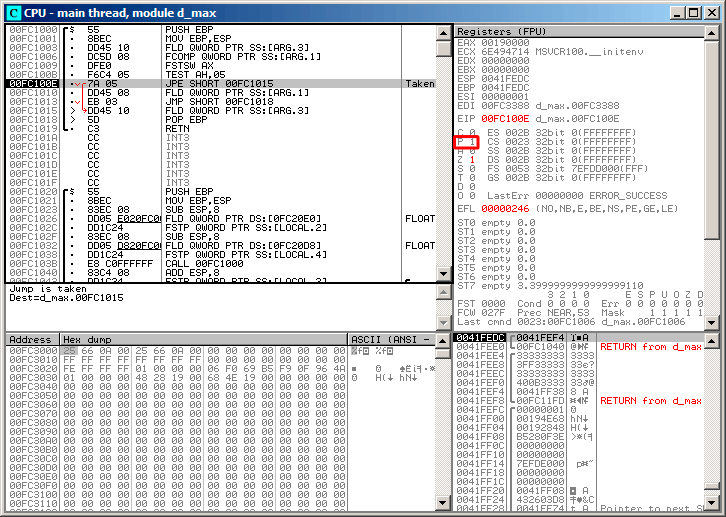
\includegraphics[scale=\FigScale]{patterns/12_FPU/3_comparison/x86/MSVC/olly1_4.png}
\caption{\olly: \TEST is executed}
\label{fig:FPU_comparison_case1_olly4}
\end{figure}

The \GTT{PF} flag is set to 1.

Indeed: the number of bits set in 0 is 0 and 0 is an even number.
\olly disassembles \INS{JP} as \ac{JPE}---they are synonyms.
And it is about to trigger now.

\clearpage
\ac{JPE} triggered, \FLD loads the value of $b$ (3.4) in \ST{0}:

\begin{figure}[H]
\centering
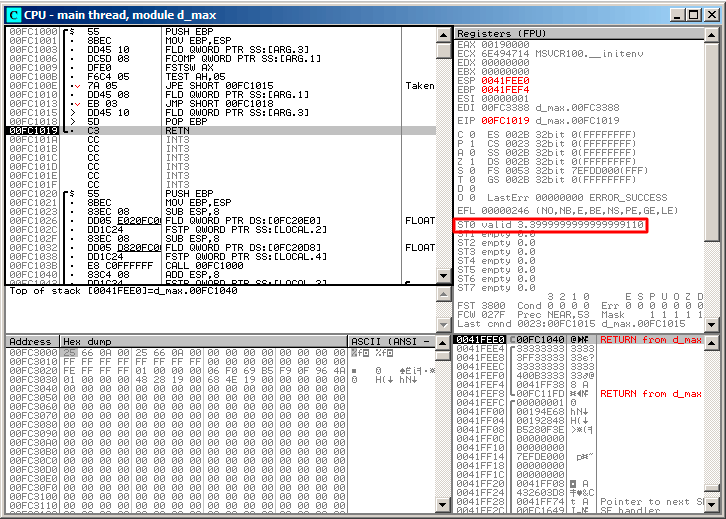
\includegraphics[scale=\FigScale]{patterns/12_FPU/3_comparison/x86/MSVC/olly1_5.png}
\caption{\olly: second \FLD is executed}
\label{fig:FPU_comparison_case1_olly5}
\end{figure}

The function finishes its work.

\clearpage
\myparagraph{Second \olly example: a=5.6 and b=-4}

Let's load example into \olly:

\begin{figure}[H]
\centering
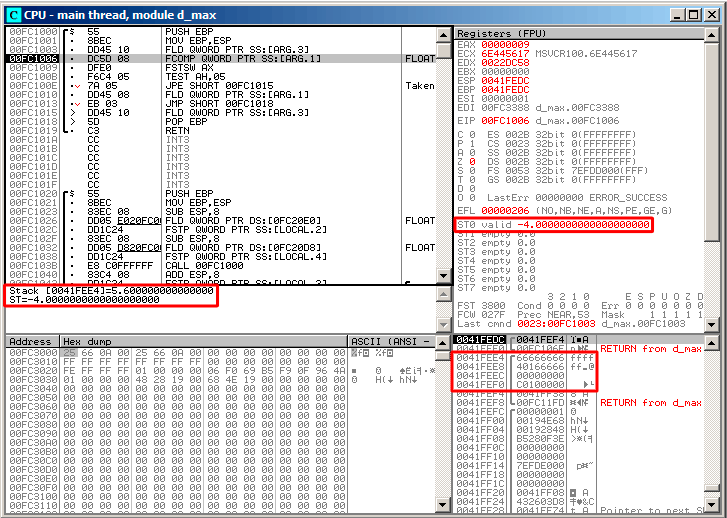
\includegraphics[scale=\FigScale]{patterns/12_FPU/3_comparison/x86/MSVC/olly2_1.png}
\caption{\olly: first \FLD executed}
\label{fig:FPU_comparison_case2_olly1}
\end{figure}

Current function arguments: $a=5.6$ and $b=-4$.
$b$ (-4) is already loaded in \ST{0}.
\FCOMP about to execute now. 
\olly shows the second \FCOMP argument, which is in stack right now.

\clearpage
\FCOMP executed:

\begin{figure}[H]
\centering
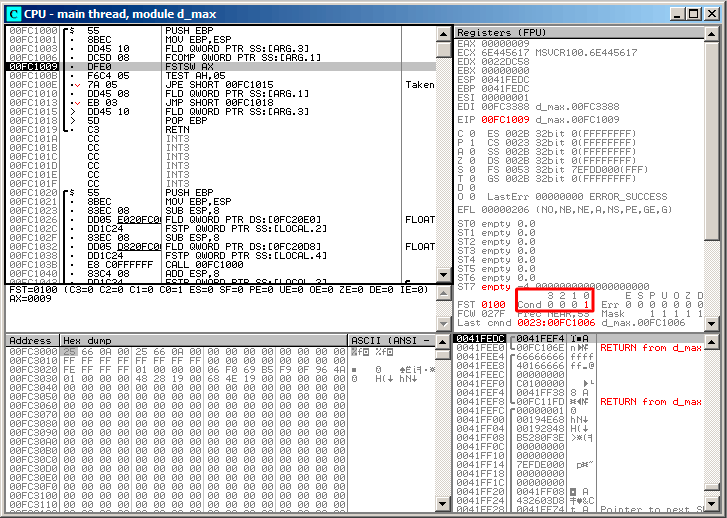
\includegraphics[scale=\FigScale]{patterns/12_FPU/3_comparison/x86/MSVC/olly2_2.png}
\caption{\olly: \FCOMP executed}
\label{fig:FPU_comparison_case2_olly2}
\end{figure}

We see the state of the \ac{FPU}'s condition flags: all zeroes except \Czero.

\clearpage
\FNSTSW executed:

\begin{figure}[H]
\centering
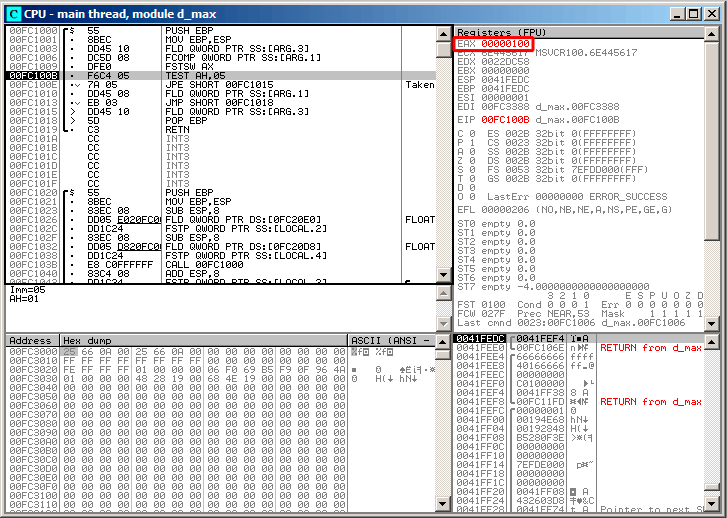
\includegraphics[scale=\FigScale]{patterns/12_FPU/3_comparison/x86/MSVC/olly2_3.png}
\caption{\olly: \FNSTSW executed}
\label{fig:FPU_comparison_case2_olly3}
\end{figure}

We see that the \GTT{AX} register contains \GTT{0x100}: the \Czero flag is at the 16th bit.

\clearpage
\TEST executed:

\begin{figure}[H]
\centering
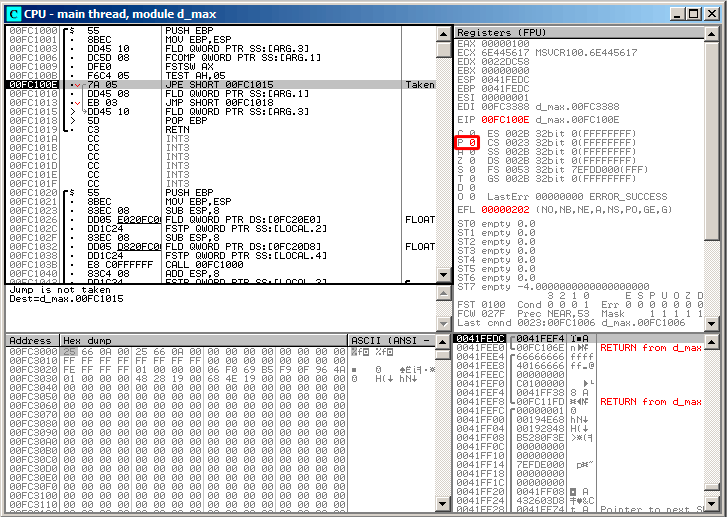
\includegraphics[scale=\FigScale]{patterns/12_FPU/3_comparison/x86/MSVC/olly2_4.png}
\caption{\olly: \TEST executed}
\label{fig:FPU_comparison_case2_olly4}
\end{figure}

The \GTT{PF}  flag is cleared.
Indeed: 

the count of bits set in \GTT{0x100} is 1 and 1 is an odd number.
\ac{JPE} is being skipped now.

\clearpage
\ac{JPE} wasn't triggered, so \FLD loads the value of $a$ (5.6) in \ST{0}:

\begin{figure}[H]
\centering
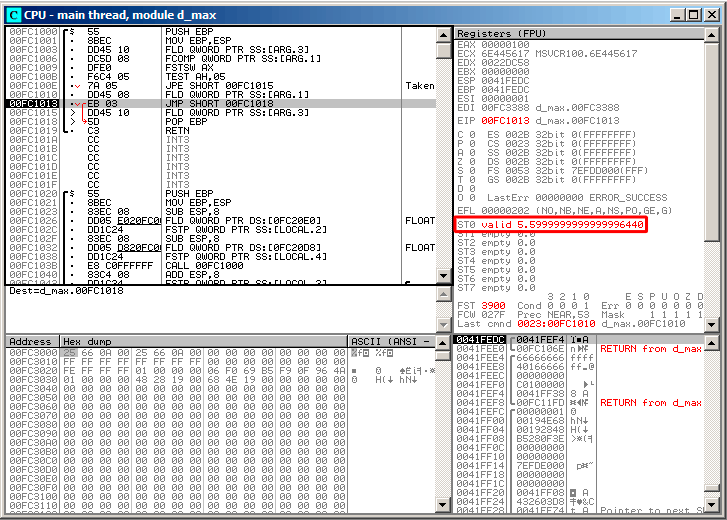
\includegraphics[scale=\FigScale]{patterns/12_FPU/3_comparison/x86/MSVC/olly2_5.png}
\caption{\olly: second \FLD executed}
\label{fig:FPU_comparison_case2_olly5}
\end{figure}

The function finishes its work.
